% Options for packages loaded elsewhere
\PassOptionsToPackage{unicode}{hyperref}
\PassOptionsToPackage{hyphens}{url}
%
\documentclass[
]{book}
\usepackage{amsmath,amssymb}
\usepackage{iftex}
\ifPDFTeX
  \usepackage[T1]{fontenc}
  \usepackage[utf8]{inputenc}
  \usepackage{textcomp} % provide euro and other symbols
\else % if luatex or xetex
  \usepackage{unicode-math} % this also loads fontspec
  \defaultfontfeatures{Scale=MatchLowercase}
  \defaultfontfeatures[\rmfamily]{Ligatures=TeX,Scale=1}
\fi
\usepackage{lmodern}
\ifPDFTeX\else
  % xetex/luatex font selection
\fi
% Use upquote if available, for straight quotes in verbatim environments
\IfFileExists{upquote.sty}{\usepackage{upquote}}{}
\IfFileExists{microtype.sty}{% use microtype if available
  \usepackage[]{microtype}
  \UseMicrotypeSet[protrusion]{basicmath} % disable protrusion for tt fonts
}{}
\makeatletter
\@ifundefined{KOMAClassName}{% if non-KOMA class
  \IfFileExists{parskip.sty}{%
    \usepackage{parskip}
  }{% else
    \setlength{\parindent}{0pt}
    \setlength{\parskip}{6pt plus 2pt minus 1pt}}
}{% if KOMA class
  \KOMAoptions{parskip=half}}
\makeatother
\usepackage{xcolor}
\usepackage{color}
\usepackage{fancyvrb}
\newcommand{\VerbBar}{|}
\newcommand{\VERB}{\Verb[commandchars=\\\{\}]}
\DefineVerbatimEnvironment{Highlighting}{Verbatim}{commandchars=\\\{\}}
% Add ',fontsize=\small' for more characters per line
\usepackage{framed}
\definecolor{shadecolor}{RGB}{248,248,248}
\newenvironment{Shaded}{\begin{snugshade}}{\end{snugshade}}
\newcommand{\AlertTok}[1]{\textcolor[rgb]{0.94,0.16,0.16}{#1}}
\newcommand{\AnnotationTok}[1]{\textcolor[rgb]{0.56,0.35,0.01}{\textbf{\textit{#1}}}}
\newcommand{\AttributeTok}[1]{\textcolor[rgb]{0.13,0.29,0.53}{#1}}
\newcommand{\BaseNTok}[1]{\textcolor[rgb]{0.00,0.00,0.81}{#1}}
\newcommand{\BuiltInTok}[1]{#1}
\newcommand{\CharTok}[1]{\textcolor[rgb]{0.31,0.60,0.02}{#1}}
\newcommand{\CommentTok}[1]{\textcolor[rgb]{0.56,0.35,0.01}{\textit{#1}}}
\newcommand{\CommentVarTok}[1]{\textcolor[rgb]{0.56,0.35,0.01}{\textbf{\textit{#1}}}}
\newcommand{\ConstantTok}[1]{\textcolor[rgb]{0.56,0.35,0.01}{#1}}
\newcommand{\ControlFlowTok}[1]{\textcolor[rgb]{0.13,0.29,0.53}{\textbf{#1}}}
\newcommand{\DataTypeTok}[1]{\textcolor[rgb]{0.13,0.29,0.53}{#1}}
\newcommand{\DecValTok}[1]{\textcolor[rgb]{0.00,0.00,0.81}{#1}}
\newcommand{\DocumentationTok}[1]{\textcolor[rgb]{0.56,0.35,0.01}{\textbf{\textit{#1}}}}
\newcommand{\ErrorTok}[1]{\textcolor[rgb]{0.64,0.00,0.00}{\textbf{#1}}}
\newcommand{\ExtensionTok}[1]{#1}
\newcommand{\FloatTok}[1]{\textcolor[rgb]{0.00,0.00,0.81}{#1}}
\newcommand{\FunctionTok}[1]{\textcolor[rgb]{0.13,0.29,0.53}{\textbf{#1}}}
\newcommand{\ImportTok}[1]{#1}
\newcommand{\InformationTok}[1]{\textcolor[rgb]{0.56,0.35,0.01}{\textbf{\textit{#1}}}}
\newcommand{\KeywordTok}[1]{\textcolor[rgb]{0.13,0.29,0.53}{\textbf{#1}}}
\newcommand{\NormalTok}[1]{#1}
\newcommand{\OperatorTok}[1]{\textcolor[rgb]{0.81,0.36,0.00}{\textbf{#1}}}
\newcommand{\OtherTok}[1]{\textcolor[rgb]{0.56,0.35,0.01}{#1}}
\newcommand{\PreprocessorTok}[1]{\textcolor[rgb]{0.56,0.35,0.01}{\textit{#1}}}
\newcommand{\RegionMarkerTok}[1]{#1}
\newcommand{\SpecialCharTok}[1]{\textcolor[rgb]{0.81,0.36,0.00}{\textbf{#1}}}
\newcommand{\SpecialStringTok}[1]{\textcolor[rgb]{0.31,0.60,0.02}{#1}}
\newcommand{\StringTok}[1]{\textcolor[rgb]{0.31,0.60,0.02}{#1}}
\newcommand{\VariableTok}[1]{\textcolor[rgb]{0.00,0.00,0.00}{#1}}
\newcommand{\VerbatimStringTok}[1]{\textcolor[rgb]{0.31,0.60,0.02}{#1}}
\newcommand{\WarningTok}[1]{\textcolor[rgb]{0.56,0.35,0.01}{\textbf{\textit{#1}}}}
\usepackage{longtable,booktabs,array}
\usepackage{calc} % for calculating minipage widths
% Correct order of tables after \paragraph or \subparagraph
\usepackage{etoolbox}
\makeatletter
\patchcmd\longtable{\par}{\if@noskipsec\mbox{}\fi\par}{}{}
\makeatother
% Allow footnotes in longtable head/foot
\IfFileExists{footnotehyper.sty}{\usepackage{footnotehyper}}{\usepackage{footnote}}
\makesavenoteenv{longtable}
\usepackage{graphicx}
\makeatletter
\def\maxwidth{\ifdim\Gin@nat@width>\linewidth\linewidth\else\Gin@nat@width\fi}
\def\maxheight{\ifdim\Gin@nat@height>\textheight\textheight\else\Gin@nat@height\fi}
\makeatother
% Scale images if necessary, so that they will not overflow the page
% margins by default, and it is still possible to overwrite the defaults
% using explicit options in \includegraphics[width, height, ...]{}
\setkeys{Gin}{width=\maxwidth,height=\maxheight,keepaspectratio}
% Set default figure placement to htbp
\makeatletter
\def\fps@figure{htbp}
\makeatother
\setlength{\emergencystretch}{3em} % prevent overfull lines
\providecommand{\tightlist}{%
  \setlength{\itemsep}{0pt}\setlength{\parskip}{0pt}}
\setcounter{secnumdepth}{5}
\usepackage{booktabs}
\ifLuaTeX
  \usepackage{selnolig}  % disable illegal ligatures
\fi
\usepackage[]{natbib}
\bibliographystyle{plainnat}
\usepackage{bookmark}
\IfFileExists{xurl.sty}{\usepackage{xurl}}{} % add URL line breaks if available
\urlstyle{same}
\hypersetup{
  pdftitle={{[}Name of Workshop{]}{[}Year{]}},
  pdfauthor={Instructors: {[}list instructor names here{]}},
  hidelinks,
  pdfcreator={LaTeX via pandoc}}

\title{{[}Name of Workshop{]}{[}Year{]}}
\author{Instructors: {[}list instructor names here{]}}
\date{{[}Insert dates of the workshop{]}}

\begin{document}
\maketitle

{
\setcounter{tocdepth}{1}
\tableofcontents
}
\part{Introduction}\label{part-introduction}

\chapter{Welcome}\label{welcome}

Welcome to CBW's {[}workshop name, year{]} Workshop!

Put some introductory content here. (ex. links to bioinformatics.ca, general info)

\chapter{Course Schedule}\label{course-schedule}

Copy paste a table into \url{https://www.tablesgenerator.com/markdown_tables} (select convert to markdown) to create a table in markdown.

\section{Pre-workshop Materials}\label{pre-workshop-materials}

Click \href{insert\%20link\%20here}{here} for your prework!

\section{Computing Setup \& Downloads}\label{computing-setup-downloads}

Insert downloads (ex. datasets) or other tech instructions here (ex. AWS Instructions)

\section{Meet Your Faculty}\label{meet-your-faculty}

Here's your team!

\subsection{Instructor, TA, \ldots{}}\label{instructor-ta}

\begin{quote}
Job Title
Company/University/\ldots{}
Location

--- contact information
\end{quote}

{[}insert description of the person{]}

\subsection{Michelle Brazas, PhD}\label{michelle-brazas-phd}

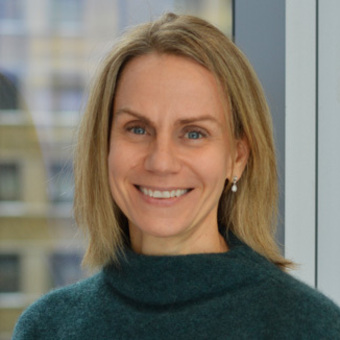
\includegraphics{./img/faculty/michelle-brazas.jpg}\\

\begin{quote}
Scientific Director
Canadian Bioinformatics Workshops (CBW)
Toronto, ON, CA

--- \href{mailto:support@bioinformatics.ca}{\nolinkurl{support@bioinformatics.ca}}
\end{quote}

Dr.~Michelle Brazas is the Associate Director for Adaptive Oncology at the Ontario Institute for
Cancer Research (OICR), and acting Scientific Director at Bioinformatics.ca. Previously, Dr.
Brazas was the Program Manager for Bioinformatics.ca and a faculty member in
Biotechnology at BCIT. Michelle co-founded and runs the Toronto Bioinformatics User Group
(TorBUG) now in its 11th season, and plays an active role in the International Society of
Computational Biology where she sits on the Board of Directors and Executive Board.

\subsection{Nia Hughes (she/her)}\label{nia-hughes-sheher}

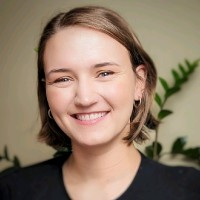
\includegraphics{./img/faculty/nia-hughes.jpeg}\\

\begin{quote}
Program Manager, Bioinformatics.ca
Ontario Institute for Cancer Research
Toronto, ON, Canada

--- \href{mailto:nia.hughes@oicr.on.ca}{\nolinkurl{nia.hughes@oicr.on.ca}}
\end{quote}

Nia is the Program Manager for Bioinformatics.ca, where she coordinates the Canadian
Bioinformatics Workshop Series. Prior to starting at OICR, she completed her M.Sc. in
Bioinformatics from the University of Guelph in 2020 before working there as a
bioinformatician studying epigenetic and transcriptomic patterns across maize varieties.

\section{Class Photo}\label{class-photo}

\textless- Replace the file address to your actual class photo file location

\part{Modules}\label{part-modules}

\chapter{Module 1}\label{module-1}

Welcome to module 1!

\section{Lecture}\label{lecture}

Here is an example of a pdf embedded:

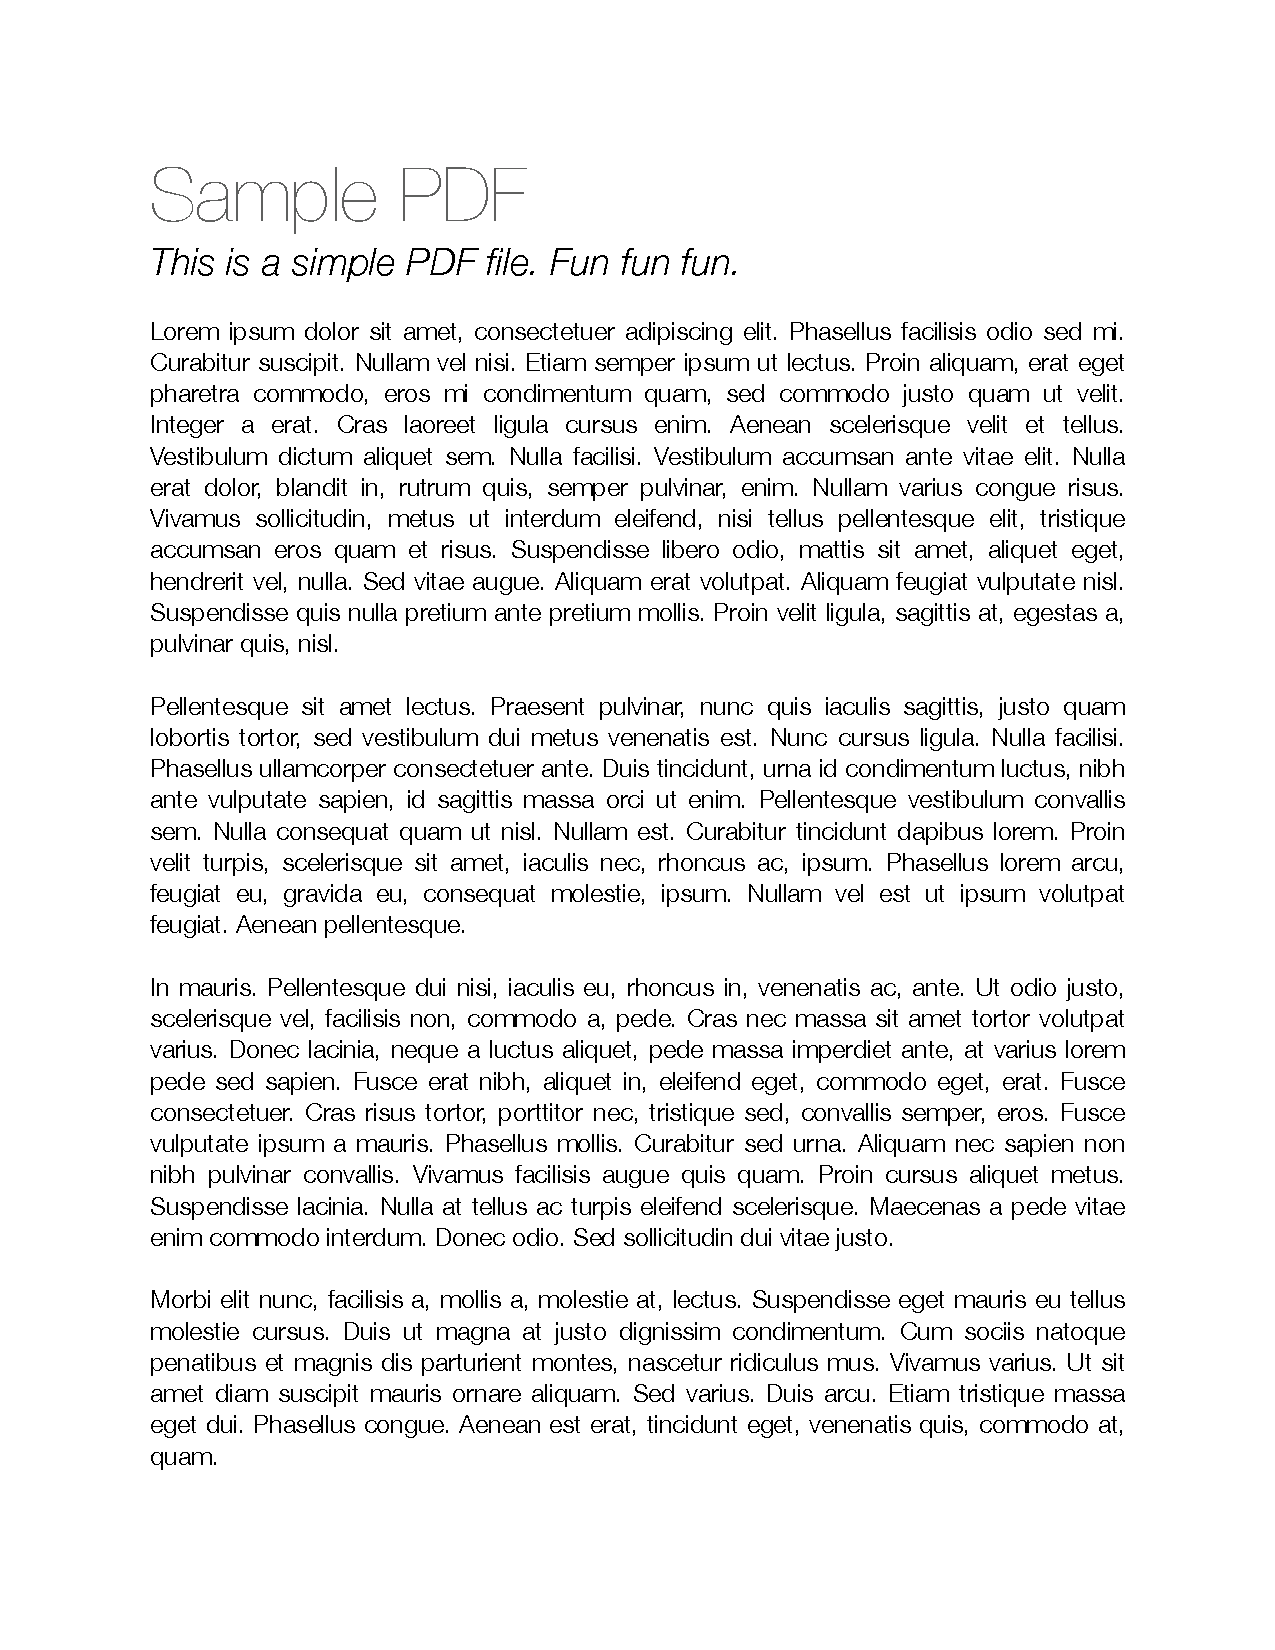
\includegraphics[width=1\textwidth,height=9.375in]{content-files/sample-pdf.pdf}~

Here is an example of a YouTube video embedded:

\^{} HEIGHT HAS A BUG

\subsection{Downloads}\label{downloads}

{[}insert your downloads for this module here (ex. datasets){]}

\section{Lab}\label{lab}

{[}Your lab here{]}

\begin{Shaded}
\begin{Highlighting}[]
\CommentTok{\# Your R code here}

\CommentTok{\# For example:}
\NormalTok{x }\OtherTok{\textless{}{-}} \DecValTok{42}
\NormalTok{x}
\end{Highlighting}
\end{Shaded}

\begin{verbatim}
## [1] 42
\end{verbatim}

\begin{Shaded}
\begin{Highlighting}[]
\CommentTok{\# Your python code here}

\CommentTok{\# For example:}
\BuiltInTok{print}\NormalTok{(}\StringTok{"hello world"}\NormalTok{)}
\end{Highlighting}
\end{Shaded}

\begin{verbatim}
## hello world
\end{verbatim}

\begin{Shaded}
\begin{Highlighting}[]
\CommentTok{\# Your bash code here}

\CommentTok{\# For example:}
\BuiltInTok{pwd}
\end{Highlighting}
\end{Shaded}

\begin{verbatim}
## /Users/jqiu/Documents/CBWgithub/cbw-dev-templates-docs/bookdown-template
\end{verbatim}

Try running these code ``chunks'' by pressing the green (left-pointing) triangle next to your code chunks.

You will see the code run in the console and the output provided below the code chunk.

The output of the code will also be produced under the code chunk on your website page.

\chapter{Module 2}\label{module-2}

\section{Lecture}\label{lecture-1}

\section{Lab}\label{lab-1}

put some example of producing images, show chunk options

\texttt{\{r,\ pressure-plot,\ echo=FALSE\},\ \ plot(pressure)}

\begin{itemize}
\tightlist
\item
  include formatting options
\end{itemize}

  \bibliography{book.bib,packages.bib}

\end{document}
